\documentclass[12pt,a4paper]{article}
\usepackage{tikz,amsmath, amssymb,bm,color,graphicx}
\usepackage[margin=1cm]{geometry}
\usetikzlibrary{calc,shapes,arrows,matrix,arrows.meta,positioning,decorations.pathreplacing,decorations.markings}

\tikzset{ midd/.style={
		decoration={
			markings,
			mark=at position 0.5 with {%
				\makebox[4pt][r]{\arrow{triangle 45}},
			},
		},
		postaction={decorate},{Circle[]}-{Circle[]}
	},}%
\begin{document}
	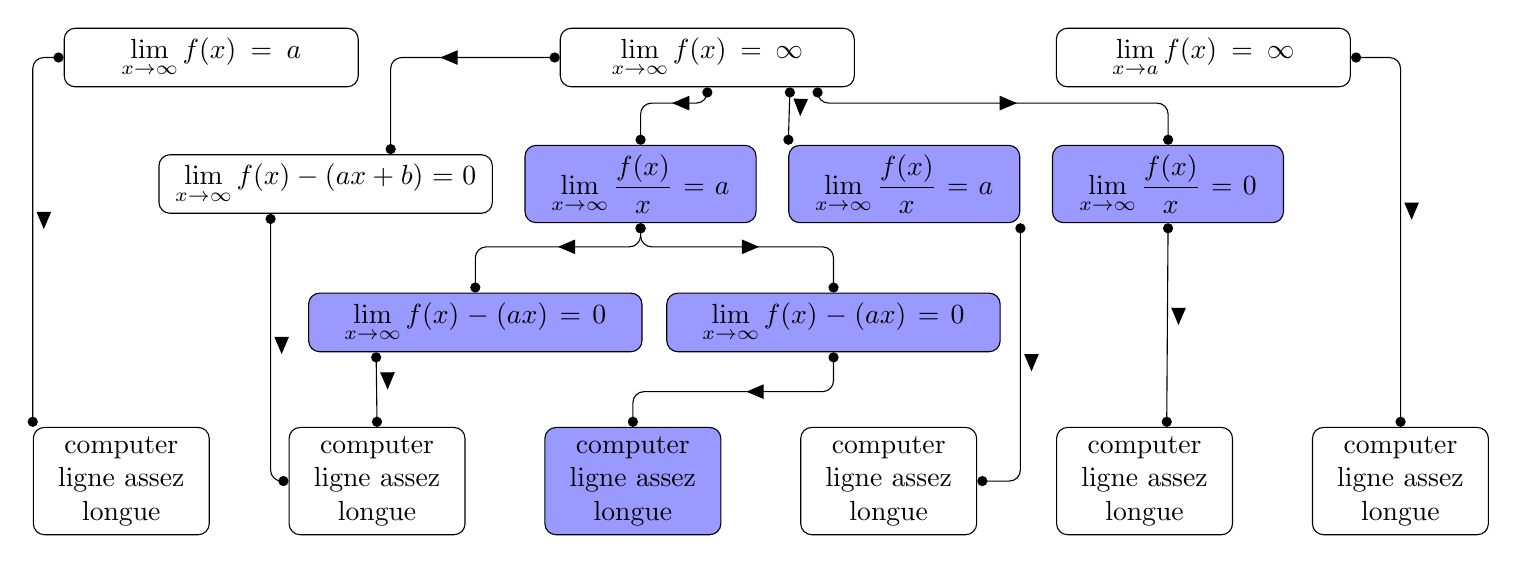
\begin{tikzpicture}[yscale=2,xscale=1.4,rounded corners=4pt]
		% xscale et yscale permettent d'ajuster largeur et hauteur
		% positionner les nœuds
		\node(a) at (-0.5,0)[rectangle,draw,,text width=3.5 cm,,text centered] {$\lim\limits_{x \to \infty} f(x)=a$};
		\node(b) at (4,0)[rectangle,draw,,text width=3.5 cm,,text centered] {$\lim\limits_{x \to \infty} f(x)=\infty$};
		\node(c) at (8.5,0)[rectangle,draw,,text width=3.5 cm,,text centered] {$\lim\limits_{x \to a} f(x)=\infty$};
		%
		\node(d) [below left=1.2cm of b ,rectangle,draw,text width=4 cm,text centered] {$\lim\limits_{x \to \infty} f(x)-(ax+b)=0$};
		\node(e) [right=0.4cm of d ,rectangle,draw,text width=2.7cm,text centered,fill=blue!40] {$\lim\limits_{x \to \infty} \dfrac{f(x)}{x}=a$};
		\node(f) [right=0.4cm of e ,rectangle,draw,text width=2.7cm,text centered,fill=blue!40] {$\lim\limits_{x \to \infty} \dfrac{f(x)}{x}=a$};
		\node(g) [right=0.4cm of f ,rectangle,draw,text width=2.7cm,text centered,fill=blue!40] {$\lim\limits_{x \to \infty} \dfrac{f(x)}{x}=0$};
		%
		\node(h) [below =1cm of d ,rectangle,draw,text width=4cm,text centered,xshift=1.9cm,fill=blue!40,] {$\lim\limits_{x \to \infty} f(x)-(ax)=0$};
		\node(i) [right=0.3cm of h,rectangle,draw,text width=4cm,text centered,fill=blue!40] {$\lim\limits_{x \to \infty} f(x)-(ax)=0$};
		%
		\node(j) [below left=1.34cm of h ,rectangle,draw,text width=2cm,text centered,xshift=-0.3cm] {computer\\ligne assez longue};
		\node(k) [right=1cm of j ,rectangle,draw,text width=2cm,text centered] {computer\\ligne assez longue};
		\node(l) [right=1cm of k ,rectangle,draw,text width=2cm,text centered,fill=blue!40] {computer\\ligne assez longue};
		\node(m) [right=1cm of l ,rectangle,draw,text width=2cm,text centered] {computer\\ligne assez longue};
		\node(n) [right=1cm of m ,rectangle,draw,text width=2cm,text centered] {computer\\ligne assez longue};
		\node(o) [right=1cm of n ,rectangle,draw,text width=2cm,text centered] {computer\\ligne assez longue};
		%%%arrow%%%%%%%%%%%%%%%%%%%
		%%%%%%%%%%%%%%%%%%
		\draw[midd](a.west)-|(j.north west);
		\draw[midd]([xshift=-0.5cm]d.south)|-(k.west);
		\draw[midd](b)-|([xshift=2.5cm]d);
		\draw[midd](b.south)--([yshift=-0.1cm]b.south)-|(e.north);
		\draw[midd ]([xshift=0.75cm]b.south)--(f.north west);
		\draw[midd]([xshift=1cm]b.south)--([xshift=1cm,yshift=-0.1cm]b.south)-|(g);
		%
		\draw[midd](e.south)--([yshift=-0.15cm]e.south)-|(h.north);
		\draw[midd](e.south)--([yshift=-0.15cm]e.south)-|(i.north);
		\draw[midd](f.south east)|-(m.east);
		\draw[midd]([xshift=-0.9cm]h.south)--(k.north);
		\draw[midd](i.south)--([yshift=-0.25cm]i.south)-|(l.north);
		\draw[midd](g.south)--([xshift=0.2cm]n.north);
		\draw[midd](c.east)-|(o.north);
	\end{tikzpicture}
\end{document}
